% -----------------
% abnTeX2: Modelo de Trabalho Acadêmico (tese de doutorado, dissertação de
% mestrado e trabalhos monográficos em geral) em conformidade com 
% ABNT NBR 14724:2011: Informação e documentação - Trabalhos acadêmicos -
% Apresentação
% -----------------

\documentclass[
	% -- opções da classe memoir --
	12pt,                     % tamanho da fonte
	openright,                % capítulos começam em pág ímpar (insere página vazia caso preciso)
	oneside,                  % twoside para impressão em verso e anverso. Oposto a oneside
	a4paper,                  % tamanho do papel. 
  % -- opções da classe abntex2 --
	% chapter=TITLE,          % títulos de capítulos convertidos em letras maiúsculas
	% section=TITLE,          % títulos de seções convertidos em letras maiúsculas
	% subsection=TITLE,       % títulos de subseções convertidos em letras maiúsculas
	% subsubsection=TITLE,    % títulos de subsubseções convertidos em letras maiúsculas
  % -- opções do pacote babel --
	english,                  % idioma adicional para hifenização
	% french,                 % idioma adicional para hifenização
	% spanish,                % idioma adicional para hifenização
	brazil                    % o último idioma é o principal do documento
]{abntex2}

% --- 
% Pacotes básicos 
\usepackage{lmodern}          % Usa a fonte Latin Modern		
\usepackage[T1]{fontenc}      % Seleção de códigos de fonte.
\usepackage[utf8]{inputenc}   % Codificação do documento (conversão automática dos acentos)
\usepackage{lastpage}         % Usado pela Ficha catalográfica
\usepackage{indentfirst}      % Indenta o primeiro parágrafo de cada seção.
\usepackage{color}            % Controle das cores
\usepackage{graphicx}         % Inclusão de gráficos
\usepackage{microtype}        % para melhorias de justificação
\usepackage{colortbl}         % Colorir linhas de tabelas
\usepackage[portuges]{datetime2}
% \DTMlangsetup[portuges]{showdayofmonth=false}
		
% ---
% Pacotes adicionais, usados apenas no âmbito do Modelo Canônico do abnteX2
\usepackage{lipsum}                           % para geração de dummy text

% ---
% Pacotes de citações
\usepackage[brazilian,hyperpageref]{backref}  % Paginas com as citações na bibl
\usepackage[num]{abntex2cite}                 % Citações padrão ABNT

% --- 
% CONFIGURAÇÕES DE PACOTES

% Configurações do pacote backref
% Usado sem a opção hyperpageref de backref
\renewcommand{\backrefpagesname}{Citado na(s) página(s):~}

% Texto padrão antes do número das páginas
\renewcommand{\backref}{}

% Define os textos da citação
\renewcommand*{\backrefalt}[4]{
	\ifcase #1
		Nenhuma citação no texto.
	\or
		Citado na página #2.
	\else
		Citado #1 vezes nas páginas #2.
	\fi}

% ---
% Informações de dados para CAPA e FOLHA DE ROSTO

\titulo{Titulo do Trabalho}
\autor{Nome do Autor Aqui}
\local{Campina Grande}
\data{\the\year{}}
\orientador{Orientador}
\newcommand{\instituto}{
  Instituto Federal de Educação, Ciência e Tecnologia\\
  da Paraíba - Campus Campina Grande\\
  Curso Superior de Tecnologia em Telemática
}
\tipotrabalho{Trabalho de conclusão de curso}
% O preambulo deve conter o tipo do trabalho, o objetivo, 
% o nome da instituição e a área de concentração 
\preambulo{Monografia apresentada à Coordenação doCurso de Telemática do IFPB - CampusCampina  Grande,  como  requisito  parcialpara conclusão do curso de Tecnologia emTelemática.}

\renewcommand{\imprimircapa}{
  \begin{capa}
    \center

    \begin{figure}
      \begin{center}
        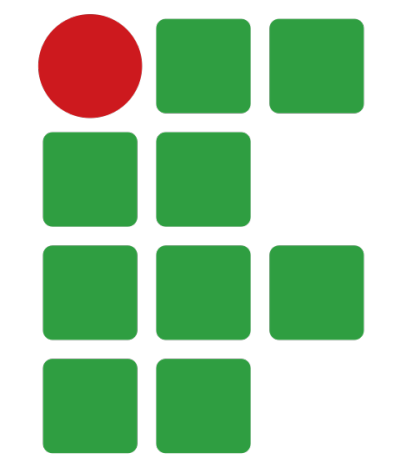
\includegraphics[width=1.8cm]{./assets/logo-ifpb.png}
      \end{center}
    \end{figure}

    \ABNTEXchapterfont \large \MakeUppercase{\instituto}

    \vspace*{2.5cm}

    \ABNTEXchapterfont \large \MakeUppercase{\imprimirautor}

    \vfill
    \begin{center}
      \ABNTEXchapterfont \bfseries \large \MakeUppercase{\imprimirtitulo}
    \end{center}
    \vfill
    % \vspace*{6.25cm}

    \large \imprimirlocal
    \par
    \large \imprimirdata
    \vspace*{1cm}
  \end{capa}
}


% ---
% Configurações de aparência do PDF final

\definecolor{blue}{RGB}{41,5,195}  % alterando o aspecto da cor azul

% informações do PDF
\makeatletter
\hypersetup{
  % pagebackref=true,
  pdftitle={\@title}, 
  pdfauthor={\@author},
  pdfsubject={\imprimirpreambulo},
  pdfcreator={LaTeX with abnTeX2},
  pdfkeywords={abnt}{latex}{abntex}{abntex2}{trabalho acadêmico}, 
  colorlinks=true,          % false: boxed links; true: colored links
  linkcolor=blue,           % color of internal links
  citecolor=blue,           % color of links to bibliography
  filecolor=magenta,        % color of file links
  urlcolor=blue,
  bookmarksdepth=4
}
\makeatother

% --- 
% Espaçamentos entre linhas e parágrafos 

\setlength{\parindent}{1.3cm} % O tamanho do parágrafo

% Controle do espaçamento entre um parágrafo e outro:
\setlength{\parskip}{0.2cm} % Tente também \onelineskip

\makeindex  % Compila o índice

\newcommand{\comentario}[1]{{\color{green}[Comentario] #1}}

\citebrackets[] % fazer com que as citações dentro do texto virem colchetes

% ---
% Início do documento
\begin{document}
\frenchspacing  % Retira espaço extra obsoleto entre as frases.

% ---
% ELEMENTOS PRÉ-TEXTUAIS
% ---
\pretextual
\imprimircapa
\imprimirfolhaderosto*

% Isto é um exemplo de Ficha Catalográfica, ou ``Dados internacionais de
% catalogação-na-publicação''. Você pode utilizar este modelo como referência. 
% Porém, provavelmente a biblioteca da sua universidade lhe fornecerá um PDF
% com a ficha catalográfica definitiva após a defesa do trabalho. Quando estiver
% com o documento, salve-o como PDF no diretório do seu projeto e substitua todo
% o conteúdo de implementação deste arquivo pelo comando abaixo:
%
% \begin{fichacatalografica}
%     \includepdf{fig_ficha_catalografica.pdf}
% \end{fichacatalografica}

\begin{fichacatalografica}
  \vspace*{\fill}                 % Posição vertical
  \hrule                          % Linha horizontal
  \begin{center}                  % Minipage Centralizado
    \begin{minipage}[c]{12.5cm}   % Largura

      \imprimirautor

      \hspace{0.5cm} \imprimirtitulo  / \imprimirautor. --
      \imprimirlocal, \imprimirdata-

      \hspace{0.5cm} \pageref{LastPage} p. : il. (algumas color.) ; 30 cm.\\

      \hspace{0.5cm} \imprimirorientadorRotulo~\imprimirorientador\\

      \hspace{0.5cm}
      \parbox[t]{\textwidth}{\imprimirtipotrabalho~--~\imprimirinstituicao,
        \imprimirdata.}\\

      \hspace{0.5cm}
      1. Palavra-chave1.
      2. Palavra-chave2.
      I. Orientador.
      II. Universidade xxx.
      III. Faculdade de xxx.
      IV. Título\\

      \hspace{8.75cm} CDU 02:141:005.7\\

    \end{minipage}
  \end{center}
  \hrule
\end{fichacatalografica}
       % Ficha bibliografica
\begin{errata}
  Elemento opcional da \citeonline[4.2.1.2]{NBR14724:2011}. Exemplo:

  \vspace{\onelineskip}

  FERRIGNO, C. R. A. \textbf{Tratamento de neoplasias ósseas apendiculares com
  reimplantação de enxerto ósseo autólogo autoclavado associado ao plasma
  rico em plaquetas}: estudo crítico na cirurgia de preservação de membro em
  cães. 2011. 128 f. Tese (Livre-Docência) - Faculdade de Medicina Veterinária e
  Zootecnia, Universidade de São Paulo, São Paulo, 2011.

  \begin{table}[htb]
    \center
    \footnotesize
    \begin{tabular}{|p{1.4cm}|p{1cm}|p{3cm}|p{3cm}|}
      \hline
      \textbf{Folha} & \textbf{Linha} & \textbf{Onde se lê} & \textbf{Leia-se} \\
      \hline
      1              & 10             & auto-conclavo       & autoconclavo     \\
      \hline
    \end{tabular}
  \end{table}

\end{errata}
        % Errata
% Isto é um exemplo de Folha de aprovação, elemento obrigatório da NBR
% 14724/2011 (seção 4.2.1.3). Você pode utilizar este modelo até a aprovação
% do trabalho. Após isso, substitua todo o conteúdo deste arquivo por uma
% imagem da página assinada pela banca com o comando abaixo:
%
% \includepdf{folhadeaprovacao_final.pdf}
%

\begin{folhadeaprovacao}
  \begin{center}
    {\ABNTEXchapterfont\large\imprimirautor}

    \vspace*{\fill}\vspace*{\fill}
    \begin{center}
      \ABNTEXchapterfont \bfseries \Large \imprimirtitulo
    \end{center}
    \vspace*{\fill}

    \hspace{.45\textwidth}
    \begin{minipage}{.5\textwidth}
      \imprimirpreambulo
    \end{minipage}
    \vspace*{\fill}

    % Trabalho aprovado. \imprimirlocal, \today:
  \end{center}

  \assinatura{\textbf{\imprimirorientador} \\ Orientador}
  \assinatura{\textbf{Professor} \\ Membro da Banca}
  \assinatura{\textbf{Professor} \\ Membro da Banca}
  %\assinatura{\textbf{Professor} \\ Convidado 3}
  %\assinatura{\textbf{Professor} \\ Convidado 4}

  \begin{center}
    \vspace*{0.5cm}
    {\large\imprimirlocal}
    \par
    {\large\imprimirdata}
    \vspace*{1cm}
  \end{center}

\end{folhadeaprovacao}
      % Folha de aprovação
\begin{dedicatoria}
  \vspace*{\fill}
  \centering
  \noindent
  \textit{ Este trabalho é dedicado às crianças adultas que,\\
    quando pequenas, sonharam em se tornar cientistas.} \vspace*{\fill}
\end{dedicatoria}
    % Dedicatória
\begin{agradecimentos}
  Os agradecimentos principais são direcionados à Gerald Weber, Miguel Frasson,
  Leslie H. Watter, Bruno Parente Lima, Flávio de Vasconcellos Corrêa, Otavio Real
  Salvador, Renato Machnievscz\footnote{Os nomes dos integrantes do primeiro
    projeto abn\TeX\ foram extraídos de
    \url{http://codigolivre.org.br/projects/abntex/}} e todos aqueles que
  contribuíram para que a produção de trabalhos acadêmicos conforme
  as normas ABNT com \LaTeX\ fosse possível.

  Agradecimentos especiais são direcionados ao Centro de Pesquisa em Arquitetura
  da Informação\footnote{\url{http://www.cpai.unb.br/}} da Universidade de
  Brasília (CPAI), ao grupo de usuários
  \emph{latex-br}\footnote{\url{http://groups.google.com/group/latex-br}} e aos
  novos voluntários do grupo
  \emph{\abnTeX}\footnote{\url{http://groups.google.com/group/abntex2} e
    \url{http://abntex2.googlecode.com/}}~que contribuíram e que ainda
  contribuirão para a evolução do \abnTeX.

\end{agradecimentos}
        % Agradecimentos
\begin{epigrafe}
  \vspace*{\fill}
  \begin{flushright}
    \textit{``Não vos amoldeis às estruturas deste mundo, \\
      mas transformai-vos pela renovação da mente, \\
      a fim de distinguir qual é a vontade de Deus: \\
      o que é bom, o que Lhe é agradável, o que é perfeito.\\
      (Bíblia Sagrada, Romanos 12, 2)}
  \end{flushright}
\end{epigrafe}
      % Epígrafe
% resumo em português
\setlength{\absparsep}{18pt} % ajusta o espaçamento dos parágrafos do resumo
\begin{resumo}
  Segundo a \citeonline[3.1-3.2]{NBR6028:2003}, o resumo deve ressaltar o
  objetivo, o método, os resultados e as conclusões do documento. A ordem e a extensão
  destes itens dependem do tipo de resumo (informativo ou indicativo) e do
  tratamento que cada item recebe no documento original. O resumo deve ser
  precedido da referência do documento, com exceção do resumo inserido no
  próprio documento. (\ldots) As palavras-chave devem figurar logo abaixo do
  resumo, antecedidas da expressão Palavras-chave:, separadas entre si por
  ponto e finalizadas também por ponto.

  \textbf{Palavras-chaves}: latex. abntex. editoração de texto.
\end{resumo}

% resumo em inglês
\begin{resumo}[Abstract]
  \begin{otherlanguage*}{english}
    This is the english abstract.

    \vspace{\onelineskip}

    \noindent
    \textbf{Key-words}: latex. abntex. text editoration.
  \end{otherlanguage*}
\end{resumo}

% resumo em francês 
% \begin{resumo}[Résumé]
%   \begin{otherlanguage*}{french}
%     Il s'agit d'un résumé en français.

%     \textbf{Mots-clés}: latex. abntex. publication de textes.
%   \end{otherlanguage*}
% \end{resumo}

% % resumo em espanhol
% \begin{resumo}[Resumen]
%   \begin{otherlanguage*}{spanish}
%     Este es el resumen en español.

%     \textbf{Palabras clave}: latex. abntex. publicación de textos.
%   \end{otherlanguage*}
% \end{resumo}
     % Resumos
% ---
% Lista de ilustrações
\pdfbookmark[0]{\listfigurename}{lof}
\listoffigures*
\cleardoublepage

% ---
% Lista de tabelas
\pdfbookmark[0]{\listtablename}{lot}
\listoftables*
\cleardoublepage

% ---
% Lista de abreviaturas e siglas
\begin{siglas}
  \item[ABNT] Associação Brasileira de Normas Técnicas
  \item[abnTeX] ABsurdas Normas para TeX
\end{siglas}

% ---
% Lista de símbolos
\begin{simbolos}
  \item[$ \Gamma $] Letra grega Gama
  \item[$ \Lambda $] Lambda
  \item[$ \zeta $] Letra grega minúscula zeta
  \item[$ \in $] Pertence
\end{simbolos}
         % Listas

% ---
% Sumario
\pdfbookmark[0]{\contentsname}{toc}
\tableofcontents*
\cleardoublepage

% ---
% ELEMENTOS TEXTUAIS
% ---
\textual

% ---
% Introdução (exemplo de capítulo sem numeração, mas presente no Sumário)
\chapter[Introdução]{Introdução}
\label{cap:intro}

PRINCIPAIS PROBLEMAS:

\begin{itemize}
    \item definição do tema e do problema
    \item não se delimita o que é estudado, o corte da pesquisa e o problema
    \item mostrar só “APLICAÇÃO DA CIÊNCIA DA COMPUTAÇÃO EM ALGO”, mas o trabalho com o tema deve contribuir para uma divisão temática da área. Por exemplo:
\end{itemize}

SUGESTÃO DE ROTEIRO:
\begin{enumerate}
    \item Contextualização do assunto com sua importância, significado para a área ligada com seu estudo, atualidade etc.

          “Nos dias de hoje, um dos assuntos mais discutidos na área de redes tem sido...”\\“Atualmente, o emprego de metodologias ativas com o uso de tecnologia tem...”\\ “Pesquisas sobre visualização de dados são muito relevantes para o desenvolvimento de aplicações em XXXX, pois...”

    \item CUIDADO!!!! Afirmações categóricas devem ter referências. Por exemplo, se você começar dizendo que a área de machine learning é muito importante para o diagnóstico médico, precisa citar um autor que dê respaldo.

    \item Conceitos (poucos – uma a três citações porque serão mais bem desenvolvidos na fundamentação teórica)

    \item Mostre como os autores abordam problemas relacionados ao assunto que você vai tratar

    \item Identifique lacunas, incompletudes, situações específicas e melhorias que poderiam ser feitas no modo como os autores têm tratado o problema

    \item Mostre como vai ATACAR UM PROBLEMA! Você pode dizer que um autor deixou de lado algo importante, que pode complementar uma solução, que pode abordar um problema de modo mais específico para uma situação particular etc. Aqui temos o “LEITMOTIV” do seu trabalho: um norte que deve guiar você em cada autor que for usar, metodologia que for aplicar, modos de analisar etc.

\end{enumerate}

Este documento e seu código-fonte são exemplos de referência de uso da classe \textsf{abntex2} e do pacote \textsf{abntex2cite}. O documento exemplifica a elaboração de trabalho acadêmico (tese, dissertação e outros do gênero) produzido conforme a ABNT NBR 14724:2011 \emph{Informação e documentação - Trabalhos acadêmicos - Apresentação}.

A expressão ``Modelo Canônico'' é utilizada para indicar que \abnTeX\ não é modelo específico de nenhuma universidade ou instituição, mas que implementa tão somente os requisitos das normas da ABNT. Uma lista completa das normas observadas pelo \abnTeX\ é apresentada em \citeonline{abntex2classe}.


Este documento deve ser utilizado como complemento dos manuais do \abnTeX\ \cite{abntex2classe,abntex2cite,abntex2cite-alf} e da classe \textsf{memoir} \cite{memoir}.

Esperamos, sinceramente, que o \abnTeX\ aprimore a qualidade do trabalho que você produzirá, de modo que o principal esforço seja concentrado no principal: na contribuição científica.

Exemplo de tabela: a Tabela~\ref{tab:dicas} mostra a pergunta que deve nortear o desenvolvimento de cada seção deste trabalho.

% Please add the following required packages to your document preamble:
% \usepackage[table,xcdraw]{xcolor}
% If you use beamer only pass "xcolor=table" option, i.e. \documentclass[xcolor=table]{beamer}
\begin{table}[h!]
    \small
    \caption{Orientações sucintas para desenvolvimento de cada seção deste trabalho.}
    \begin{tabular}{|l|l|}
        \hline
        \rowcolor[gray]{0.9}
        \multicolumn{1}{|c|}{\cellcolor[gray]{0.9}\textbf{Elemento textual}} & \textbf{Qual a pergunta que norteia seu desenvolvimento} \\ \hline
        \textbf{\begin{tabular}[c]{@{}l@{}}Introdução (Motivação e\\ definição do problema)\end{tabular}}                                   & \begin{tabular}[c]{@{}l@{}}O que? - definir claramente o problema a ser abordado na pesquisa;\\ Por quê? - indicar a importância de resolver o problema\end{tabular}                                \\ \hline
        \textbf{\begin{tabular}[c]{@{}l@{}}Introdução (Objetivos gerais e\\ específicos)\end{tabular}}                                   & \begin{tabular}[c]{@{}l@{}}Para que? - definir qual o objetivo geral da pesquisa;\\ Quais as etapas? - definir objetivos específicos que ajudarão a\\ atingir o objetivo geral\end{tabular}                                \\ \hline
        \textbf{\begin{tabular}[c]{@{}l@{}}Introdução (Estrutura do\\ documento)\end{tabular}}                                   & \begin{tabular}[c]{@{}l@{}}Como o texto está organizado e apresentado?\\ O que será discutido em cada seção?\end{tabular}                                \\ \hline
        \textbf{Trabalhos relacionados}                                      & \begin{tabular}[c]{@{}l@{}}Baseado em que? O que já foi feito? - discutir o estado da arte e\\ o que já foi estudado sobre o problema\end{tabular}                                \\ \hline
        \textbf{Descrição da proposta}                                       & \begin{tabular}[c]{@{}l@{}}Qual a aplicabilidade? – a solução para o problema servirá a\\ que propósitos? onde será aplicável?\\ Como? - Indicar através de quais procedimentos, instrumentos\\ e mecanismos a investigação será conduzida;\\ O que já foi conseguido até aqui?\end{tabular}                               \\ \hline
        \textbf{\begin{tabular}[c]{@{}l@{}}Propostas para Continuação \\ da Pesquisa, Cronograma\end{tabular}}                                  & \begin{tabular}[c]{@{}l@{}}O que ainda falta?\\ Em quanto tempo? - definir atividades e indicar quando tempo \\ estima-se empreender em cada uma delas\end{tabular}                               \\ \hline
    \end{tabular}
    \label{tab:dicas}
\end{table}


% --------------------------------------


\section{Justificativa e Relevância do Trabalho}
\label{sec:justificativa}
Explicar porque foi escolhido esse tema, qual sua importância para a área, etc...

DEVE:

Demonstrar a relevância da pesquisa em questão. Informar que contribuições o estudo trará para a compreensão, a intervenção ou a solução do problema – justificativas incluem mostrar as várias contribuições do trabalho: educacionais, científico-tecnológicas, relação com outros trabalhos, retorno social e para a comunidade acadêmica etc.

EVENTUALMENTE ACRESCENTAR:
\begin{itemize}
    \item por qual razão se deve investir tempo e dinheiro em sua pesquisa
    \item a origem do tema retomando sua explicação
    \item relevâncias:
          \begin{itemize}
              \item científica
              \item social
              \item específica
          \end{itemize}
\end{itemize}

% --------------------------------------


\section{Objetivos}
\label{sec:objetivos}
\subsection{Objetivo Geral}
\label{subsec:objGeral}

O objetivo principal deste trabalho ......
OBJETIVO GERAL deve ter:
\begin{itemize}
    \item o máximo onde quero chegar – PENSE, em atingindo o objetivo, o que efetivamente obterá?
    \item envolve compreender algo, mas não pode ser só isso\\
          CUIDADO!!!!!!! “Estudar” (e outros VERBOS GERAIS) são o objetivo do aluno e não do trabalho!!\\
          NO MESTRADO, DEVE-SE PENSAR MAIS NOS OBJETIVOS de PESQUISA E NÃO SÓ NOS OBJETIVOS TÉCNICOS!!!!
    \item CUIDADO para não confundir as consequências do objetivo com O SEU objetivo!
          Ex.: um sistema em geral não vai conscientizar, melhorar o ensino, tornar a empresa melhor
    \item verbos SEMPRE no infinitivo impessoal:
          “analisar, descrever, comparar, constituir, formar, ampliar, propor, melhorar” etc.
\end{itemize}


\subsection{Objetivos Específicos}
\label{subsec:objespecificos}

OBJETIVOS ESPECÍFICOS DEVEM:
\begin{itemize}
    \item ser os passos para chegar no geral
    \item o conjunto deles forma o geral
    \item pense nos passos e atividades de um videogame para ganhar (objetivo geral) um jogo
    \item verbos no infinitivo: comparar, mapear, investigar, analisar…
\end{itemize}

% --------------------------------------


\section{Metodologia}
\label{sec:metodologia}

A metodologia empregada para desenvolvimento do trabalho ....


%% ------------------------------------------------------------------------- %%


\section{Organização do Documento}
\label{sec:organizacao}

Os capítulos subsequentes estão organizados da seguinte maneira:

\begin{itemize}
    \item O conceito de ... é apresentado em detalhes no Capítulo~\ref{cap:capitulos}, incluindo uma descrição...

    \item No Capítulo \ref{cap:capitulos} é apresentada a metodologia e...

    \item As considerações finais e as propostas de continuação do trabalho são descritos no Capítulo~\ref{cap:capitulos}...
\end{itemize}



\chapter{Capítulos}
\label{cap:capitulos}

Os capítulos seguintes devem ser definidos de acordo com as especificidades de cada trabalho. Lembre de usar o comando label para referenciar os capítulos e as seções

Recomenda-se:

\begin{itemize}
  \item Fundamentação Teórica
  \item Descrição de modelos/módulos desenvolvidos
  \item Resultados Obtidos
  \item Considerações Finais
  \item Sugestões para trabalhos futuros
\end{itemize}
 % Capítulos

% ---
% Finaliza a parte no bookmark do PDF
% para que se inicie o bookmark na raiz
% e adiciona espaço de parte no Sumário
% ---

%\phantompart

% Conclusão (outro exemplo de capítulo sem numeração e presente no sumário)
\chapter{Considerações Finais}
\label{cap:conlusao}


\section{Sugestões para Trabalhos Futuros}
\label{sec:futuros}


% ---
% ELEMENTOS PÓS-TEXTUAIS
% ---
\postextual

\bibliography{abntex2-modelo-references}        % Referências bibliográficas

% ---
% Glossário
% Consulte o manual da classe abntex2 para orientações sobre o glossário.
% \glossary

\begin{apendicesenv}
  \partapendices  % Imprime uma página indicando o início dos apêndices

  \chapter{Um Apêndice}
  \label{ape:apendiceI}
  Para criar um novo apêndice utilize o comando chapter, lembre de utilizar label para referenciar.

\end{apendicesenv}
   % Apêndices
\begin{anexosenv}
  \partanexos % Imprime uma página indicando o início dos anexos

  \chapter{Um Anexo}
  \label{ape:anexoI}
  Para criar um novo anexo utilize o comando chapter, lembre de utilizar label para referenciar.

\end{anexosenv}
      % Anexos

%---
% INDICE REMISSIVO
% \phantompart
\printindex

\end{document}
